\chapter{Optimal scenario tree selection}
\label{chapter4}
In this chapter we propose an experiment to find out if it is possible to predict the optimal scenario tree structure with regard to the objective function and also propose a way to control for the complexity of the scenario tree using reinforcement learning. For this purpose, we implemented the moment matching method for generation of scenario trees, the multistage mean-CVaR model and a reinforcement learning agent.
\section{Methods}
The whole implementation was programmed in Python (\cite[Version 3.11]{python}), mathematical optimization problems were implemented in GAMS (\cite[version 40.3.0]{GAMS}) using the Python API. Data were sourced from \cite{yahoo} using the \cite[version 0.1.74]{yfinance} package. The reinforcement agent was implemented using the \textit{Stable~baselines~3} package (\cite[version 1.6.2]{stable_baselines3}) and the environment was implemented using the \textit{gym} package (\cite[version 0.21.0]{openai_gym}).

\section{Data}
\label{section:data}
For our experiments, we used data obtained from \cite{yahoo} using the \cite[version 0.1.74]{yfinance} package. We downloaded historical weekly asset price data from 1.1.2000 to 31.12.2019 for 49 financial stocks given in Table \ref{table:stock_tickers_used}. We consider two indexing sets with regard to time, set \textit{train} (from 1.1.2000 to 31.12.2009) and set \textit{test} (from 1.1.2010 to 31.12.2019) and also consider two sets of assets, set $A$ (see Table \ref{table:stock_tickers_in_set_A}) and set $B$ (see Table \ref{table:stock_tickers_in_set_B}). This yielded us four distinct sets:
\begin{itemize}
\item (\textit{train}, $A$), denoted $TrA$,
\item (\textit{test}, $A$), denoted $TeA$,
\item (\textit{train}, $B$), denoted $TrB$,
\item (\textit{test}, $B$). denoted $TeB$,
\end{itemize}
and we write the set that contains all these sets as $\kappa=\{TrA, TeA, TrB, TeB\}$.
We trained the agent on the set $TrA$ and evaluate its performance on all four sets, to evaluate whether the agent is able to:
\begin{enumerate}
\item learn something from the training data (performance on $TrA$),
\item generalise to unseen assets in the same period (performance on $TrB$),
\item generalise to the training assets in the future (performance on $TeA$),
\item generalise to unseen assets in the future (performance on $TeB$).
\end{enumerate}

\begin{rem}
We are mainly interested in the performance of the agent on sets $TrA$ and potentially also $TrB$. If the agent was able to generalise across time, this would be a breaktrough finding. Such generalisation is however unlikely due to the possibility that the distribution of the data may be different in the \textit{test} time period.
\end{rem}

We set the investment horizon to 2.5 years and from each set in $\kappa$, we needed to obtain data for the moment matching method in such a way that the scenario trees were constructed with the same investment horizon independent of the number of stages. This was achieved by splitting the investment horizon into equisized parts based on the number of stages of the tree.
Particularly, for a scenario tree with a given number of stages (denoted as $T$), we split the investment period into $T$ equisized periods (we denote the length of these periods as $\mathcal{L}$), each corresponding to the given stage.

We then used the whole available 10 years of data to estimate the distribution of returns in a period of length  $\mathcal{L}$ by splitting the 10 years of data into equisized parts of length $\mathcal{L}$, calculating simple returns (this yielded $4T$ observations), and calculating the first four sample moments and correlations between each of the assets. These moments and correlations were then used as input for the moment matching method, where the obtained moments and correlations were used for generating each stage of the scenario tree.

\begin{rem}
We considered only stagewise independent scenario trees. This is in line with the data preparation we used above, as financial returns are generally considered independent when taken over a period of time that is longer than a few days. The shortest period we used is about $6$ months (which corresponds to an investment period of 2.5 years with 5 stages), which is much longer than a few days.
\end{rem}

\section{Environment}
For the purposes of training the reinforcement agent to choose the best scenario tree structure, we adapted the well known GridWorld environment to represent iterative stage by stage building of the scenario tree.
\begin{rem}
The GridWorld environment is a well known introductory environment for training reinforcement learning agents. It consists of a $n$ by $n$ grid, $n \in \N$, where the agent starts on a given tile (a position on the grid, i.e. for example the bottom left corner) and must reach a target tile and upon reaching the tile, it receives a reward. The agent can perform 4 actions -- move up, move down, move left and move right. None of the tiles apart from the target tile return rewards. An illustration of such an environment is given in Figure \ref{fig:gridworldenv_illustration}.
\end{rem}

\begin{figure}[H]
\centering
  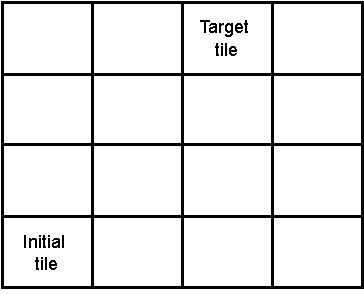
\includegraphics[width=\linewidth / 3]{../img/gridworld_env_illustration.pdf}
  \caption{Illustration of a 4 by 4 GridWorld environment. The agent starts at the Initial tile and must reach the Target tile to receive a reward.}
  \label{fig:gridworldenv_illustration}
\end{figure}

We designed and implemented a custom GridWorld environment, which we call TreeBuildingEnv.

\subsection{TreeBuildingEnv}
\label{section:treebuildingenv}
TreeBuildingEnv is an adaptation of the GridWorld environment to allow the agent to build scenario trees based on given predictors, which consist of return data of the assets that are used to build the scenario tree. 
The state is given as a 8 by 8 tree building grid (which starts filled with zeros only in the initial state) and the set of 9 predictors. 

At the beginning of each episode, between 7 and 10 assets are randomly chosen (with uniform probabilities for the number of assets) from the provided data (a set from $\kappa$) and the set of predictors is obtained at the beginning of each episode using the return data for the chosen assets for the whole time period and is constant throughout the episode. 

Each row in the tree building grid represents a part of the tree building process. The first row corresponds to the chosen number of stages in the tree. The following rows each represent the chosen branching (number of descendants of each node) in each stage, from the first to last.

In each state, the agent can take any action in the set $\{3,4,5,6,7\}$, which we from now on refer to as \textit{action set}. In the initial state, we allow the agent to perform only actions $\{3,4,5\}$ from the action set to choose the depth of tree and upon performing any of these actions, 1 is placed at the corresponding position in the first row. If the agent chooses action 6 or 7, it is forced to perform action 5\footnote{We do not allow the number of stages to be 6 or 7, as the tree is then considerably more complex and building it based on historical data and solving the resulting mean-CVaR model takes too much time for it to be practical for our experiments. The action 5 is forced for the reinforcement algorithm to be able to associate action 6 and 7 with the move to a state where action 5 was chosen.}.


\begin{figure}[H]
  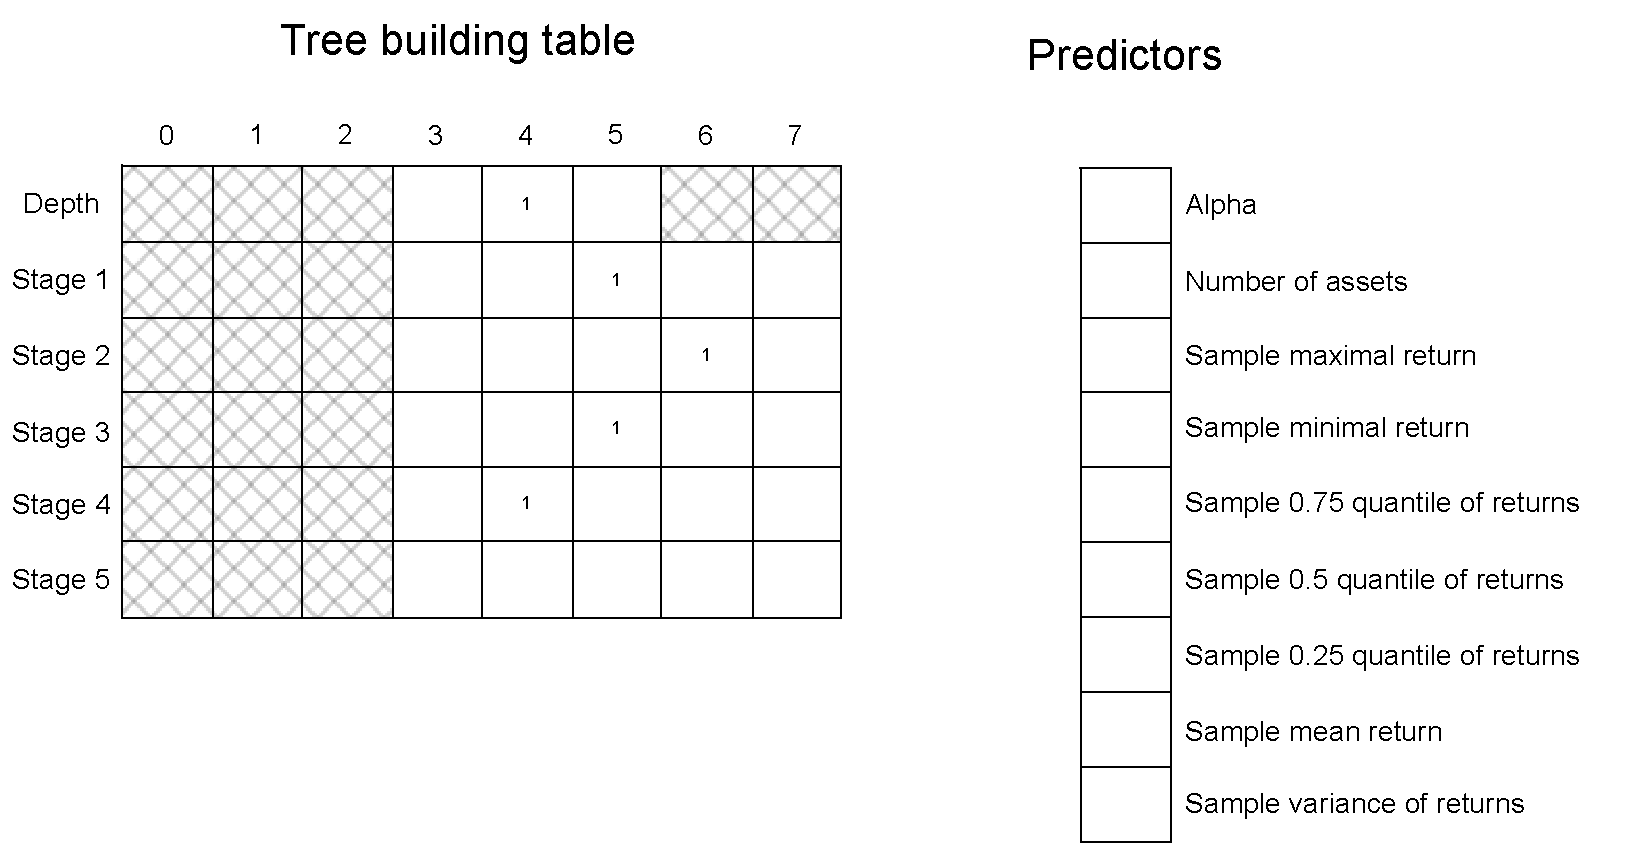
\includegraphics[width=\linewidth]{../img/Treebuildingenv_graph.pdf}
  \caption{TreeBuildingEnv. State illustration when a 4 stage tree is generated with 5 children in the first stage, 6 in the second stage, 5 in the third stage and 4 in the fourth stage. Crosshatching represents invalid actions. Predictors are represented as an empty array, in reality they are populated with numerical data on the whole period returns, see Section \ref{subsection:predictors}.}
  \label{fig:treebuildingenv}
\end{figure}


In the following states, where the agent chooses the branching (the number of descendants) in each stage, the agent can perform any action in the action set and again upon performing each action, 1 is placed at the position of the chosen action in the next row (if the action is valid, see below). 

To obtain reasonable trees, we had to constrain the size of the tree the agent can take (the maximum number of scenarios). We always require that the tree must have at least 100 scenarios and at most 1200. In each state, we check if it is possible to perform the chosen action such that a final tree that remains within these limits is possible. If it is not possible, the action is considered invalid and the agent is forced to take the maximum\footnote{we use the maximum valid action, rather than a random action, so that the agent is able to associate that an invalid action results in taking a large branching in the given stage} valid action (where valid action refers to any action for which building a tree that stays in the given limits is possible). In case the chosen action was invalid, 1 is placed at the position of the forced maximum valid action.

When the agent has taken as many actions as the chosen depth of tree, the episode ends, the mean-CVaR problem is solved using the given scenario tree structure and the obtained reward is returned (see Section \ref{section:rewards}). An illustration of the environment can be found in Figure \ref{fig:treebuildingenv}.

\subsection{Predictors}
\label{subsection:predictors}
At the beginning of each episode, between 7 and 10 assets are randomly chosen (with uniform probabilities for the number of assets) from the provided data and simple returns are calculated for the whole time range. $\alpha$ is randomly chosen with uniform probabilities from the set $\{0.8, 0.85, 0.9, 0.95\}$ and the following predictors are provided to the agent:
\begin{enumerate}
\item $\alpha$,
\item Number of sampled assets,
\item Sample maximum return,
\item Sample minimum return,
\item Sample 0.75 quantile of returns,
\item Sample 0.5 quantile of returns,
\item Sample 0.25 quantile of returns,
\item Sample mean of returns,
\item Sample variance of returns.
\end{enumerate}
The predictors are then constant throught the entire episode.

\section{Rewards}
\label{section:rewards}
A reward is returned after every action the agents takes, which is 0 for every action in states that are not terminal and at the end of the episode, in the terminal state, a reward is returned based on the solved mean-CVaR problem using the scenario tree structure that is specified by the terminal state. 
\begin{rem}
Note that the fact that the reward is sparse (reward 0 is returned when not in a terminal state) is actually quite a common occurence in reinforcement learning. Reinforcement learning is, after all, designed exactly to handle such problems.
\end{rem}

We need to specify the reward in such a way that a higher reward corresponds to a more favourable value of the objective function. We need to consider that the mean-CVaR model, as formulated in Equation \ref{eq:cvar_multistage_risk_aversion}, is formulated using the distribution of loss. This means that obtaining a smaller objective value from the mean-CVaR model is beneficial. Denoting the obtained objective value from solving the problem in Equation \ref{eq:cvar_multistage_risk_aversion} as $\varsigma$, we have to write the reward given to the agent as
\begin{equation*}
r_{terminal} = -\varsigma(s_{terminal}),
\end{equation*}
where we add the subscript $terminal$ to emphasize that this reward is calculated at the terminal state of the episode and that the reward depends on the terminal state (which represents the scenario tree structure). The objective of the agent is then to maximise $r_{terminal}$.

\subsection{Penalty}
\label{subsection:penalty_subsection}
As was mentioned in Section \ref{section:curse_od_dimensionality}, choosing a scenario tree that has too many stages and too many descendants in each stage leads to a computationally intractable problem. On the other hand, choosing a scenario tree that is too small in terms of number of stages and with too few descendants in each stage may lead to a very rough approximation of the underlying continuous distributions, leading to results with high variability. 

To ameliorate these problems, we propose to include a penalty term in the reward $r_{terminal}$ which penalizes such scenario trees. Particularly, we propose that the penalty be dependent on the number of scenarios in the tree in the last stage, i.e. the number of leaves in the tree. It is not straightforward to represent the complexity of a tree due to the multidimensional structure, but we consider that using the number of leaves provides a good enough proxy for the complexity of the scenario tree, while being simple to implement. 

Denoting the number of leaves in the tree as $\Psi$ and the penalization function as $\delta(\Psi)$, we thus propose that the reward $r_{terminal}$ be penalized as follows
\begin{equation*}
r_{terminal} = -\varsigma(s_{terminal}) - \delta(\Psi(s_{terminal})),
\end{equation*}
where the dependence of $\Psi$ on $s_{terminal}$ stresses the fact that $\Psi(s_{terminal})$ is calculated from the scenario tree structure represented in $s_{terminal}$.

To penalize the scenario tree that is too complex, we propose a linear penalization $\delta_1$
\begin{equation*}
\delta_1(\Psi) = c \frac{\Psi - \Psi_{min}}{\Psi_{max} - \Psi_{min}},
\end{equation*}
where $c$ is a chosen coefficient (which must be chosen based on the magnitude of values obtained as solutions from solving the mean-CVaR problem) and $\Psi_{max}$ and $\Psi_{min}$ are the maximum and minimum allowed number of leaves in the scenario tree respectively.

%Penalisation $\delta_1$ penalizes the complexity, but does not take into account that a small number of leaves is also detrimental. We propose another penalisation function, denoted $\delta_2$, to deal with this problem:
%\begin{equation*}
%\delta_2(\Psi) = \frac{c}{\left[(\Psi_{max}-\Psi_{min})/2\right]^2} (\Psi - \frac{\Psi_{max}+\Psi_{min}}{2})^2,
%\end{equation*}
%where again $c$ is a parameter, $\Psi_{max}$ is the maximum allowed number of leaves in the scenario tree and $\Psi_{min}$ is the minimum allowed number of leaves in the scenario tree.

%The proposed $\delta_2$ penalisation is quadratic and centered at $(\Psi_{max}+\Psi_{min})/2$ where it is 0, $c$ is the maximum penalty achieved at points $\Psi_{max}$ and $\Psi_{min}$. $c$ again is a coefficient that must be chosen based on the desired magnitude of the penalty.

Of course, this is just one possible penalization function out of infinite possibilities. The shape of the penalty function can be adjusted based on the problem at hand (and the parameter $c$ has to be adjusted as well).

In this section, we proposed only a penalization function that penalizes trees that are too complex. It might make sense to penalise also trees that are too simple, but we do not use such a penalisation in this thesis, as we already have a lower bound set on the number of leaves in the tree in the environment (the lower bound is 100 scenarios).

\section{Implementation}
\subsection{Moment matching}
\label{subsection:moment_matching}
%Gülpinar N, Rustem G, Settergren R, Simulation and Optimization Ap-
%%proaches to Scenario Generatin, Journal of Economic Dynamics & Control,
%vol. 28, Elsevier Science, 2004 - Moment matching - sequential vs whole tree
We used the moment matching method in the form given in Definition \ref{defn:moment_matching_method} sequentially on each stage using the first four sample moments and correlations which were estimated as explained in Section \ref{section:data} with one small adjustment. 

When looking at the generated scenarios for larger numbers of descendants, we noticed that usually, only 3 scenarios with positive probabilities were generated and the rest had almost zero probability. This would fundamentally change the properties of scenario trees that we want to explore (dependence of objective function on tree size), since then we might think we are using a large tree, which in reality is much smaller due to the scenarios with zero probability. 

To counteract this effect, we added the constraint $p_j \geq 0.03$ to the implementation of Definition \ref{defn:moment_matching_method}, which solved the problem. With the notation developed in Definition \ref{defn:moment_matching_method}, the model now reads
\begin{alignat}{10}
& && && \underset{\substack{p_j, x_{i,j}, \\ j \in \{1,...,N\}, i \in I}}{\min} \sum_{i\in I} \sum_{k\in \mathcal{M}} \left(m_{i,k} - M_{i,k}\right)^2 + \sum_{(i, i') \in I, i < i'}(c_{i,i'}-C_{i,i'})^2 \nonumber \\
& s.t. && \sum_{j=1}^N p_j&&=1 \nonumber \\
& && m_{i,1}&&=\sum_{j=1}^N p_jx_{i,j}, i \in I \nonumber \\
& && m_{i,k}&&=\sum_{j=1}^N p_j(x_{i,j}-m_{i,1})^k, i \in I, k>1 \nonumber \\
& && c_{i,i'}&&=\sum_{j=1}^N(x_{i,j}-m_{i,1})(x_{i',j}-m_{i',1})p_j, i,i' \in I, i<i' \nonumber
\end{alignat}
\vspace{-0.5cm}
\begin{alignat}{10}
& 0  \leq x_{i,j}, i \in I, j=1,\dots,N, \nonumber \\
& \frac{3}{100} \leq p_j \leq 1, j=1,\dots,N. \nonumber
\end{alignat}

This means that we are generating stagewise independent balanced scenario trees, where the probabilities of each child node may vary, but are at least 0.03. This may lead to the fact that we are not able to account for scenarios with very small probability, which is a limitation, as financial data distributions are generally heavy tailed. However, for the purposes of this thesis, this assumption is not too restrictive.


\subsection{Mean-CVaR model}
The mean-CVaR model was implemented exactly as given in Equation \ref{eq:cvar_multistage_risk_aversion} using the scenario tree generated from the moment matching method, where we used the risk aversion parameter $\lambda=0.3.$ \todo{how to justify choice of 0.3? Chosen by expert? @Milos Kopa}

\subsection{Reinforcement agent}
We chose to use a tried and tested implementation of state of the art algorithms in the \textit{Stable Baselines 3} library (\cite{stable_baselines3}). We experimented with multiple architectures and algorithms implemented therein, particularly A2C and PPO, while eventually settling on using PPO in the results given in Section \ref{section:experimental_results}. Here we share our experience with training the reinforcement agent.

We first experimented with the algorithms using a toy environment (TreeBuildingEnv with synthetic predictors and rewards) to obtain some semblance of how long it takes to obtain a reward better than random guessing. We experimented with several neural net architectures and found out that PPO usually outperformed A2C (converged much faster) with the same neural net architecture. 

We also experimented with neural net architectures and found that even for very simple tasks (such as learning a different action based on the value of a single predictor $p$), a very nontrivial number of neurons in the hidden layers is required for the model to be able to solve the environment. Particularly, for a deterministic toy example where $p$ was randomly sampled from the set $\{0.1, 0.2\}$ and based on the given $p$ the best number of stages to take was $3$ if $p=0.1$ and $5$ if $p=0.2$, the reinforcement agent didn't learn anything within hudreds of thousands of timesteps, unless we used an architecture with at least two hidden layers of 128 and 64 neurons respectively, where the second layer is separate for the actor and the critic (which estimate the policy and the action value). Furthermore, we used ReLu activations between each layer. 

Due to the results obtained from the synthetic toy environment, we decided to use a very similar architecture as given above, where the only change is that we use 256 and 128 neurons in the hidden layers instead of 128 and 64, as the task we are trying to solve is much more difficult and stochastic. Unfortunately, due to the computational difficulties presented in Section \ref{section:computational_difficulties}, we couldn't experiment with multiple neural network architectures by doing hyperparameter optimization on the number of neurons in each layer. The final neural net architecture that we use is visualised in Figure \ref{fig:neuralnet}. 


With regard to the hyperparameters, we used the learning rate $\varphi=0.001$, discount factor $\gamma=1$ (which is used for the calculation of $\widehat{A}(a,s)$, see \cite[Section 5]{proximal_policy_optimization}) so that the agent is not penalised for using trees with more stages and performed $192$ timesteps per update of the parameters of the neural network. Otherwise, we used the default hyperparameters, particularly $c_1=0.5$, where $c_1$ is the value function coefficient given in Equation \ref{eq:ppo_performance_measure}).

\begin{figure}[H]
  \centering
  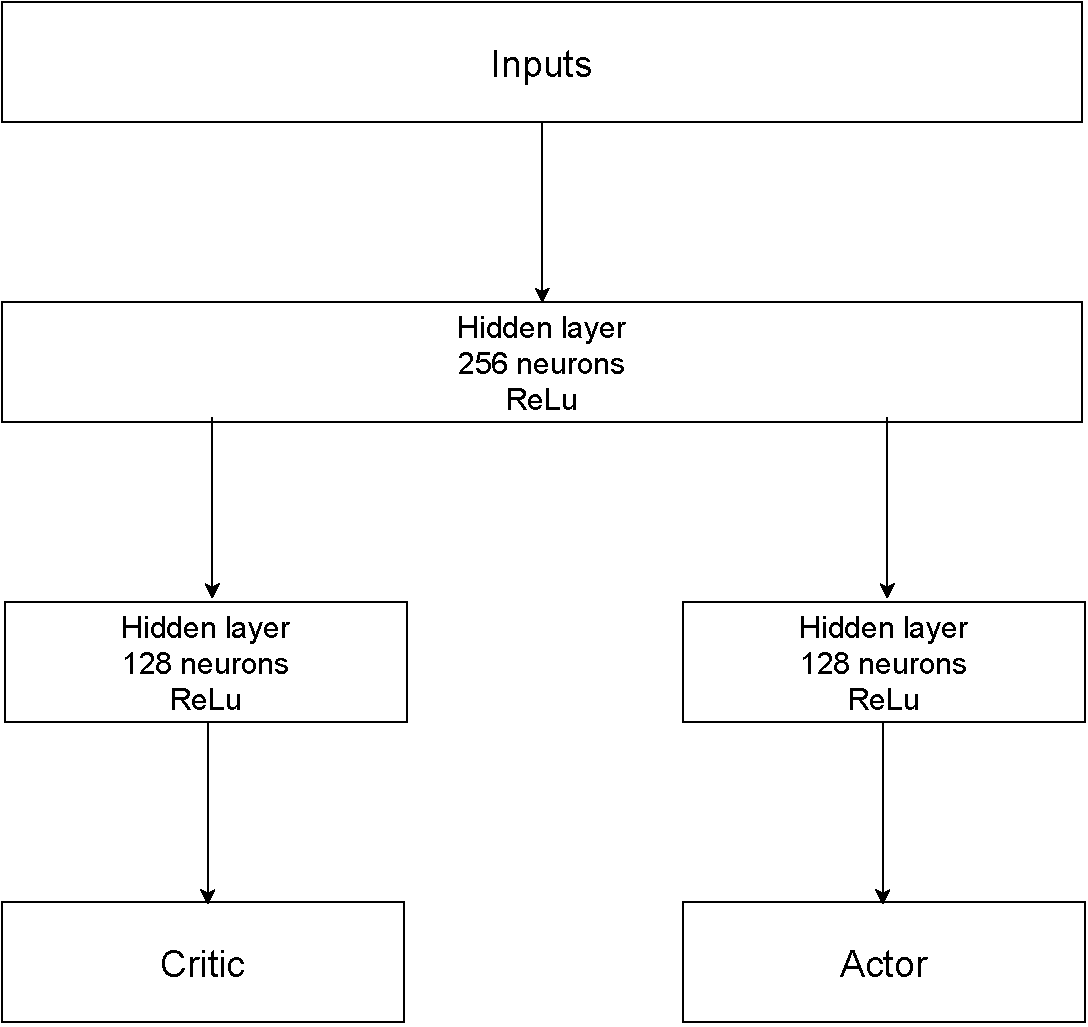
\includegraphics[width=\linewidth / 2]{../img/nn_diagram.pdf}
  \caption{Illustration of the neural network architecture used for training the PPO agent.}
  \label{fig:neuralnet}
\end{figure}

\section{Experimental results}
\label{section:experimental_results}
\input{experimental_results}

\newpage
\section{Computational difficulties}
\label{section:computational_difficulties}
The writing of this thesis has been plagued by computational difficulties from the start and we wish to share our experience with implementing all parts of this thesis here. 

First of all, the moment matching method, which seems quite easy to implement, required a significant amount of experimentation and trying different optimization frameworks and solvers to actually obtain a working implementation. We have tried several python packages with open source solvers (most notably \textit{SciPy} (\cite{scipy}) , \textit{Mystic} (\cite{mystic}) and \textit{Gekko} (\cite{gekko}) and the IPOPT solver) and none of them produced a suitable result despite correct implementation due to low strength of the open source solvers. We finally settled on using GAMS with the CONOPT solver which worked out quite nicely. This however required us to connect our Python code to GAMS using the GAMS Python API, which meant that we could not use a compute cluster due to licensing limitations. 

Since we already had the dependence on GAMS, we also implemented the mean-CVaR model in GAMS using the CPLEX solver. While the implementation itself in GAMS was not terribly difficult, bending all data in the correct way and formulating the nonanticipativity constraints correctly took significant effort.

Lastly, the reinforcement learning part. This part was plagued by slow training and therefore a significant amount of time was spent on training the models, since the dependence on GAMS didn't allow training the reinforcement agent on a compute cluster with hundreds of cores, but we were rather constrained to a personal computer with 6 cores. This was a significant limitation, since training reinforcement agents is usually very computationally intensive (e.g. the state of the art models mentioned in the beginning of Chapter \ref{chapter3} were usually trained for months on hundreds of machines).